\documentclass[10pt,a4paper]{article}
\usepackage[utf8]{inputenc} % para poder usar tildes en archivos UTF-8
\usepackage[spanish]{babel} % para que comandos como \today den el resultado en castellano
\usepackage{a4wide} % márgenes un poco más anchos que lo usual
\usepackage[conEntregas]{Sty/caratula}
\usepackage{Sty/mathtools}
\usepackage{Sty/float}
\usepackage[pdftex]{graphicx}
\usepackage{caption}
\usepackage{subcaption}
%\usepackage{Sty/algorithm2e}
\usepackage[ruled,vlined]{Sty/algorithm2e}
%Esto de abajo es para encabezado y pie de pagina
\usepackage{Sty/lastpage}
\usepackage{fancyhdr}
\usepackage{amsfonts}
\usepackage[noend]{algpseudocode}
\usepackage{enumerate} % AGREGO PARA PODER ENUMERAR LAS LINEAS DEL ALGORITMO
\usepackage{wrapfig}


\pagestyle{fancy}


\cfoot{\thepage /\pageref{LastPage} }


\begin{document}

\fecha{\today}
\materia{Organizacion del computador II}
\titulo{Trabajo Práctico III}
\grupo{Te voy a dar un Byte}

\integrante{Gonzalez Benitez, Albertito Juan}{324/14}{gonzalezjuan.ab@gmail.com}
\integrante{Lew, Axel Ariel }{225/14}{axel.lew@hotmail.com}
\integrante{Noli Villar, Juan Ignacio}{174/14}{juaninv@outlook.com}

\maketitle
\newpage
\tableofcontents	

\newpage


\subsection{Introduccion}
En este trabajo practico procederemos a realizar un sistema operativo que pueda correr un juego.

	

\newpage
\section{Ejercicio 1:}
\subsection{Introducción:}

En este ejercicio vamos a realizar la Tabla de Descriptores Globales (\textit{GDT}). Se pide que realizemos lo siguiente :

\begin{itemize}
\item [\textit{a)}] Que la tabla \textit{GDT} tenga 4 segmentos, dos para código de
nivel 0 y 3; y otros dos para datos de nivel 0 y 3. Estos segmentos deben direccionar los primeros 500MB de memoria. Por último se pide no usar las primeras siete posiciones de la \textit{GDT}, ya que se consideran utilizadas.

\item [\textit{b)}] Pasar a modo protegido y setear la pila del kernel en la dirección 0x27000. 

\item [\textit{c)}] Agregar a la \textit{GDT} un segmento adicional y escribir una rutina qe utilice este nuevo segmento para pintar la esquina superior izquierda de la pantalla.

\item [\textit{d)}] Limpiar la pantalla y pintar el área del mapa (sugerido el color gris) junto con las barras inferiores para los jugadores.
\end{itemize}

\subsection{Ítem a): Setear la \textit{GDT}}

Para este ítem completamos el archivo \textit{GDT}.c proporcionado por la catedra. En el mismo la \textit{GDT} es representada mediante un array de 30 posiciones. Cada posicion tiene la siguiente estructura.
\\

\begin{figure}[H]
\begin{center}
\minipage{0.6\textwidth}
  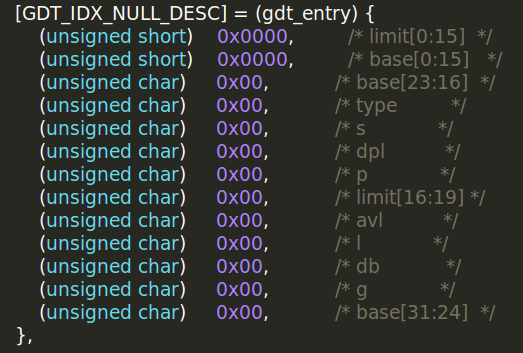
\includegraphics[width=\linewidth]{ejercicio1/GDTnula.png}
  \caption{{\small Este descriptor corresponde a la primer entrada de la \textit{GDT}}} 
\endminipage
\end{center}
\end{figure}

Como la primer posicion de la tabla \textit{GDT} debe ser corresponder a una entrada nula, llenamos la primer posicion como muestra la imagen debajo.
\\


Luego, creamos los 4 segmentos que se piden a partir de la posicion 8 de la \textit{GDT}, ya que por enunciado, no se deben tocar las primeras 7 posiciones de la table de descriptores. Mostramos en las imagenes de abajo como creamos un descriptor de datos y otro de codigos. 
\\

\begin{figure}[H]
\begin{center}
\minipage{0.5\textwidth}
  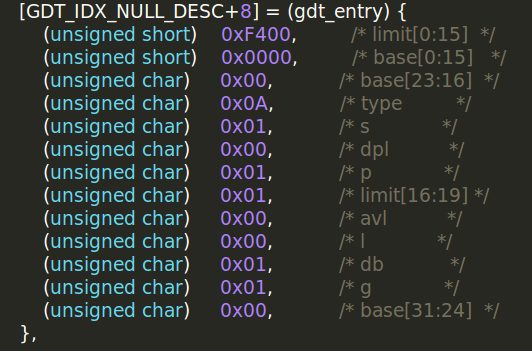
\includegraphics[width=\linewidth]{ejercicio1/GDTcodigo0.png}
  \caption{{\small Este descriptor corresponde al segmento de datos de nivel 0}} 
\endminipage
\minipage{0.5\textwidth}
  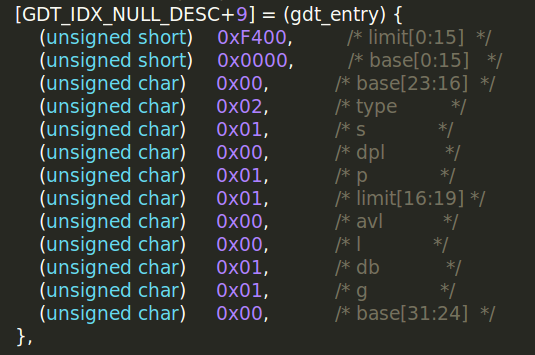
\includegraphics[width=\linewidth]{ejercicio1/GDTdatos0.png}
  \caption{{\small Este descriptor corresponde al segmento de código de nivel 0}} 
\endminipage
\end{center}
\end{figure}

Los otros dos que faltan son exactamente iguales, solo que en la linea correspondiente al nivel (dpl) ponemos 0x03, ya que corresponde al nivel 3 de prioridad.\\

Los descriptores de segmentos tienen la siguiente forma:
\\

\begin{figure}[H]
\begin{center}
\minipage{0.8\textwidth}
  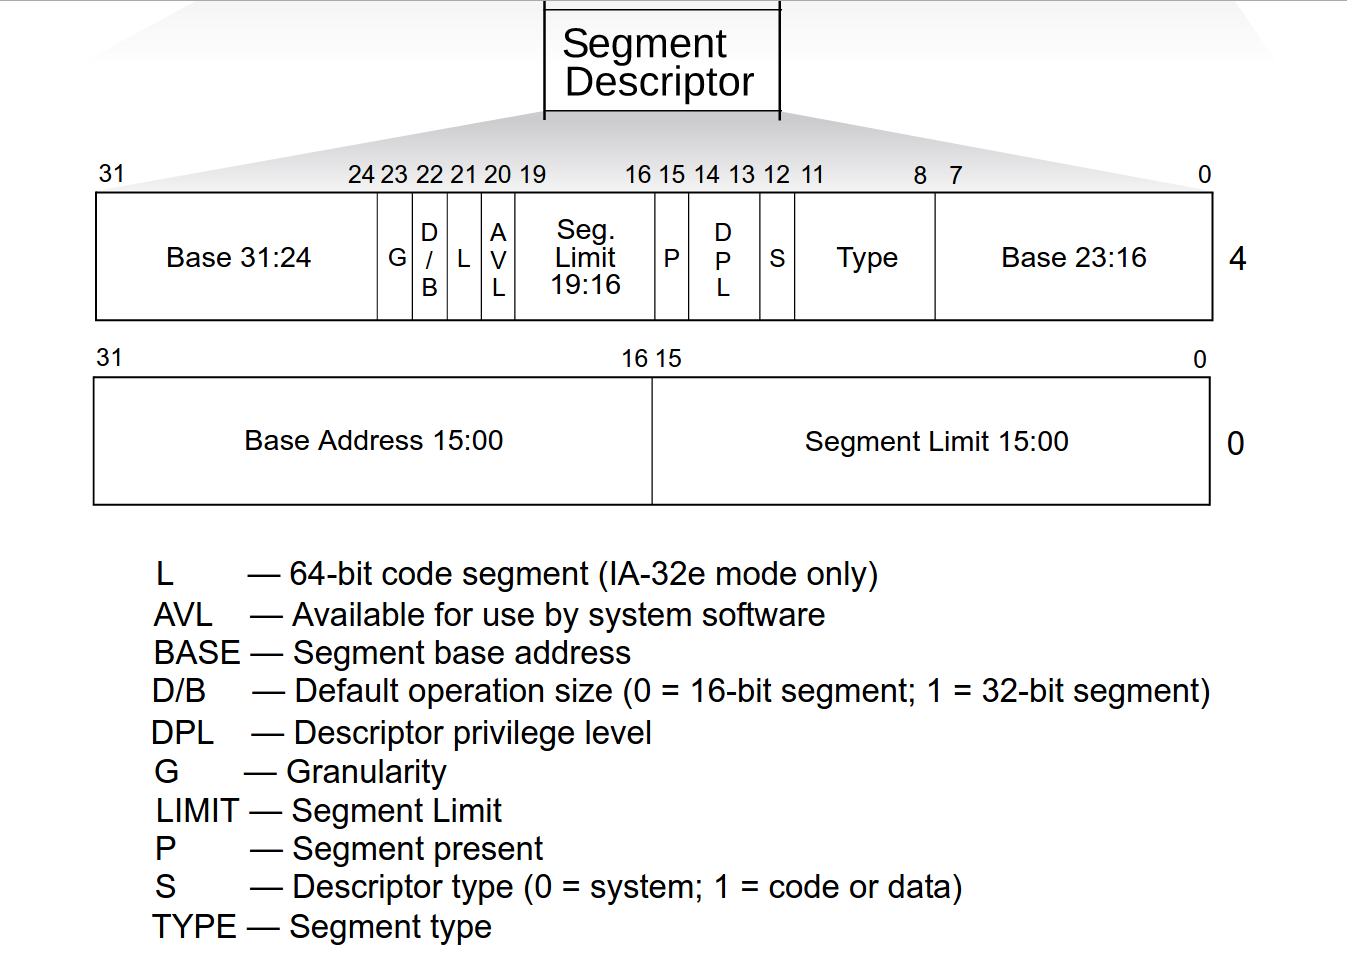
\includegraphics[width=\linewidth]{ejercicio1/estructuradescriptor.png}
  \caption{{\small Este descriptor corresponde a la primer entrada de la \textit{GDT}}} 
\endminipage
\end{center}
\end{figure}

Completamos nuestros descriptores como marcan las figuras 3 y 4 de esa forma porque:

\begin{itemize}
\item [\textit{Base:}] En el tp se pide que los descriptores direcciones los primeros 500mb de memoria. Por ende la base corresponde a la dirección 0x00000000.
\item [\textit{G:}]  Para poder direccionar 500mb, no nos alcanza la cantidad de bits que hay para el limite, por ende necesitamos activar la granularidad para poder abarcar más memoria, ya que cuando esta activada la posicion que indica el limite se multiplica por 4kb.
\item [\textit{Límite:}] Como esta activada la granularidad, podemos abarcar 500mb de memoria, el limite correspondiente a 500mb con la granularidad activada es 0x0F400.
\item [\textit{Type:}] Aqui se indica si el descriptor es de código/datos, a los correspondientes a datos les pusimos que eran de tipo 0x02 (segmento de datos de escritura/lectura) y a los de código que eran de tipo 0x0A (segmentdo de código de escritura/lectura).
\item [\textit{S:}] Con este bit se decide si es un segmento de sistema (s=0) o si son de código/data (s=1), por ende a este bit le corresponde un 0x1.
\item [\textit{Dpl:}] En esta seccion se declara el privilegio del segmento, a los que eran de nivel 0 les corresponde un 0x00 y a los de nivel 3 un 0x03
\item [\textit{P:}] Este es el bit de present. Cuando es ’1’ el segmento correspondiente esta presente en la memoria RAM. Si es ’0’, el segmento esta en la memoria virtual. Por ende lo seteamos en 1.
\item [\textit{Avl:}] Es el bit correspondiente a Available. Como no lo vamos a tener en cuenta lo dejamos en 0.
\item [\textit{L:}] Indica si el código es de 64bits o de 32. Como trabajamos en 32bits dejamos este bit en 0.
\item [\textit{D/B:}] Este bit define el tamaño de las operaciones en las que va a trabajar el procesador. De nuevo, como nos encontramos trabajando en 32bits, el tamaño de las operaciones debe ser de 32, por eso lo seteamos en 1.
\end{itemize}

\subsection{Ítem b): Pasar a modo protegido y setear la pila}

Para pasar a modo protegido realizamos los siguientes pasos:

\begin{itemize}
\item [\textit{a)}] Deshabilitamos las interrupciones, para eso utilizamos la instrucción CLI.

\item [\textit{b)}] Cargamos el registro \textit{GDTR} con la dirección base de la \textit{\textit{GDT}} utilizando la instrucción \textit{LGDT} de esta manera: 
\begin{center}
lgdt [GDT DESC]
\end{center}
Donde GDT DESC es el descriptor de la tabla.

 \item [\textit{c)}] Seteamos el bit \textit{PE} (BIT 0) del registro \textit{CR0} en 1 para pasar a modo protegido. Procedemos a hacer esto con las intrucciones:
\begin{center}
      mov eax, cr0\\
     or eax, 1   $~~~~$ \\
       mov cr0, eax
    \end{center}

\item [\textit{d)}]Realizamos un far jump para cargar en el registro \textit{CS} la dirección donde esta el segmento de código. Para esto utilizamos la instruccion: 

\begin{center}
jmp 0X40:modoprotegido
\end{center}

Donde 0x40 es la dirección donde en nuestra \textit{GDT} compienza el segmento de código y modoprotegido es una etiqueta que se encuentra imediatamente debajo de este JMP. 

\item [\textit{e)}]Cargamos los registros de segmento de la siguiente manera.

\begin{center}
   mov ax, 0x48\\
    mov ds, ax$~~~$\\
    mov ax, 0x48\\
    mov ss, ax$~~~$\\
\end{center}


\end{itemize}

Ahora que ya nos encontramos con el procesador trabajando en modo protegido, procedemos a setear la pila en la dirección 0x27000. Para eso seteamos los registros ebp y esp en la dirección 0x27000 con las siguientes instrucciones: 
\begin{center}
mov ebp, 0x27000\\
mov esp, 0x27000\\
\end{center}

\subsection{Ítem c): Agregar a la \textit{GDT}  un segmento adicional y utilizarlo como memoria de vídeo}

Para este ítem, agregamos a la \textit{GDT} el siguiente segmento, el cual direcciona a la memoria de vídeo utilizada por la pantalla (Desde 0xB8000 a 0XC000).

\begin{figure}[H]
\begin{center}
\minipage{0.5\textwidth}
  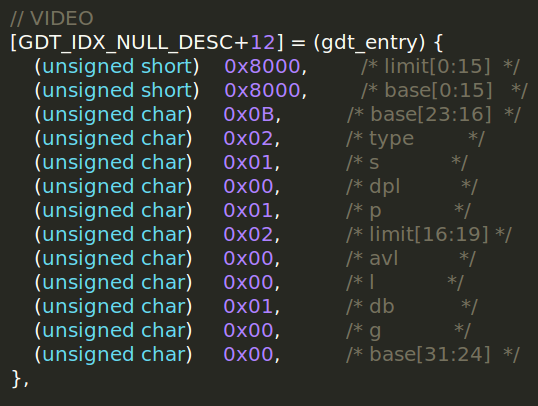
\includegraphics[width=\linewidth]{ejercicio1/memvid.png}
  \caption{{\small}} 
\endminipage
\end{center}
\end{figure}


Luego cargamos en un registro de segmento, en este caso  \textit{FS}, la posicion del segmento anterior. Por ultimo con las siguiente instrucción podemos poner en la esquina superior izquierda de la pantalla lo que querramos
\begin{center}
mov word[fs:0x00],  \textit{aimprimir}
\end{center}

Donde  \textit{aimprimir} es algo de tamaño word, y su valor es el que aparece en la esquina superior izquierda de la pantalla. Esto ocurre porque se carga el segmento que comienza en la dirección a que la dirección 0xB8000 y se le suma el offset 0 y esta es la primer dirección de la memoria de vídeo utilizada por la pantalla.\\

Si por ejemplo escribimos la siguiente línea:
\begin{center}
mov word[fs:0x00],  0xdb00
\end{center}

Obtenemos este resultado, que es lo que pedía el ejercicio.

\begin{figure}[H]
\begin{center}
\minipage{0.8\textwidth}
  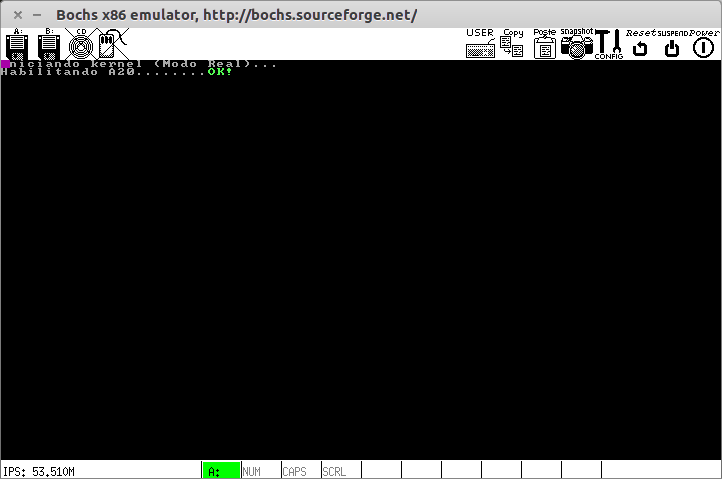
\includegraphics[width=\linewidth]{ejercicio1/esqsupizq.png}
  \caption{{\small}} 
\endminipage
\end{center}
\end{figure}

\subsection{Ítem d): Limpiar la pantalla y pintar el área del mapa}

En este punto creamos una función auxiliar en C para limpiar la pantalla. La función pinta la pantalla de gris y es la siguiente:

\begin{figure}[H]
\begin{center}
\minipage{0.3\textwidth}
  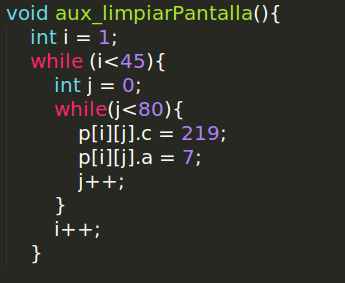
\includegraphics[width=\linewidth]{ejercicio1/limpant.png}
  \caption{{\small}} 
\endminipage
\end{center}
\end{figure}

Esta función la escribimos en \textit{screen.c} y utiliza la matriz P creada por la catedra para acceder a las posiciones de la pantalla. Estos son los resultados luego de utilizar nuestra función. \\

\begin{figure}[H]
\begin{center}
\minipage{0.8\textwidth}
  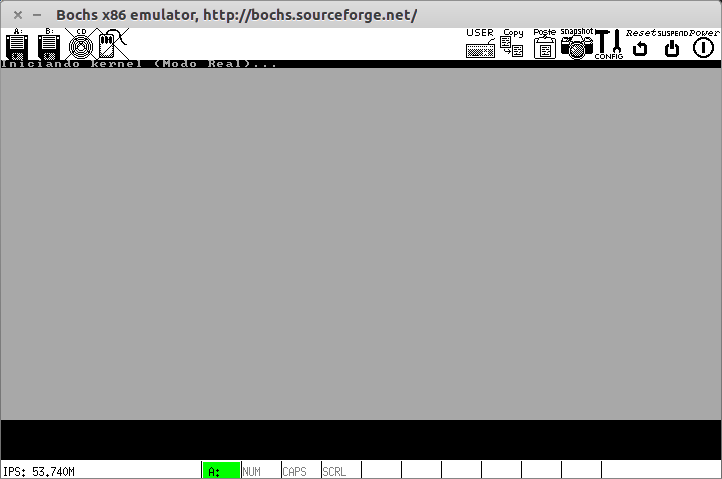
\includegraphics[width=\linewidth]{ejercicio1/pantgris.png}
  \caption{{\small}} 
\endminipage
\end{center}
\end{figure}


Para pintar el mapa utilizamos la función dada por la catedra  \textit{screen$\_$inicializar}. Para utilizar estas funciones, escribimos en \textit{kernel.asm} las siguientes lineas con el siguiente resultado:

\begin{center}
 call aux$\_$limpiarPantalla    \\
 call screen$\_$inicializar$~~~$
\end{center}

\begin{figure}[H]
\begin{center}
\minipage{0.8\textwidth}
  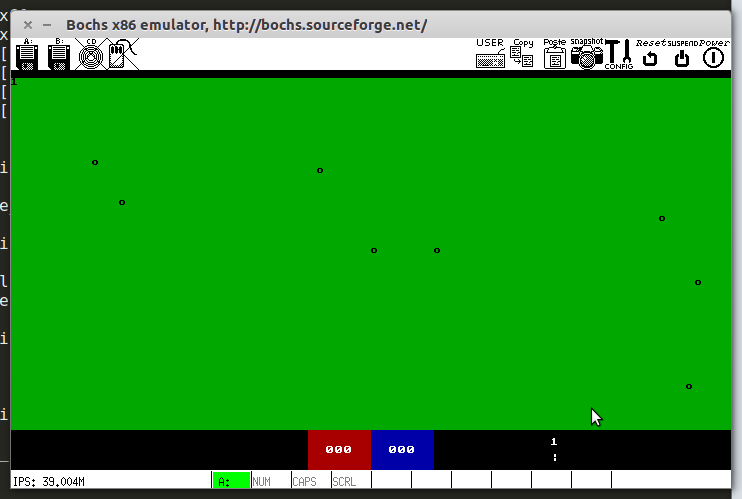
\includegraphics[width=\linewidth]{ejercicio1/mapa.png}
  \caption{{\small}} 
\endminipage
\end{center}
\end{figure}


\newpage
\section{Ejercicio 2:}
\subsection{Introducción:}

En este ejercicio vamos a setear las interrupciones basicas, osea las reservadas para el procesador. Para esto completaremos la \textit{IDT}. Se pide que realizemos lo siguiente :

\begin{itemize}
\item [\textit{a)}] Completar la \textit{IDT} de tal forma que indique por pantalla el problema que se produjo y que interrumpa la ejecución.
\item [\textit{b)}] Cargar la  \textit{IDT} y probarla.
\end{itemize}

\subsection{Ítem a): Setear la \textit{IDT}}

Para esto utilizamos los siguientes archivos dados por la catedra   \textit{idt.c}, \textit{isr.h}, \textit{isr.asm} y los completamos. 

 \subsubsection{{\large \textit{Idt.c:}}}
 En este archivo se encuentra la función \textit{IDT\_ENTRY(número, dpl)} la cual recive el numero de la interrupción y su prioridad. La misma se encontraba incompleta y necesitaba ser completada con la información necesaria. La llenamos agregandole el segmento correspondiente y los atributos correpondientes. El segmento que le correpondia se ubicaba en la direccion 0x40 (explicado en el ejercicio 1) y los atributos son los correpondientes a el valor  0x8700, ya que el formato de los atributos de una interrupcion debe ser de la siguiente forma:

 \begin{figure}[H]
\begin{center}
\minipage{0.6\textwidth}
  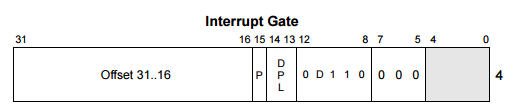
\includegraphics[width=\linewidth]{ejercicio2/interrupcion.png}
  \caption{{\small Formato de los atributos de una interrupcion} }
\endminipage
\end{center}
\end{figure}

Entonces como 0x8E00 representa en binario 1000 1110 0000 0000, tiene el formato que queremos. Ya que P debe ser 1, DPL debe ser 00, luego sigue un 0, luego D (que en este caso es 1 ya que estamos trabajando en 32bits) luego siguen dos unos y por último nueve ceros, lo cual forma el número que queremos. De esta forma nos queda la funcion \textit{IDT\_ENTRY} de la siguiente manera:

 \begin{figure}[H]
\begin{center}
\minipage{1.0\textwidth}
  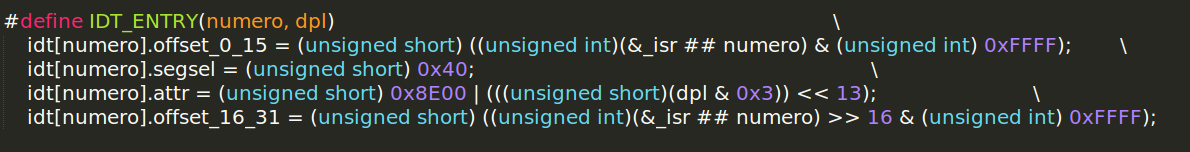
\includegraphics[width=\linewidth]{ejercicio2/idtentry.png}
  \caption{{\small Formato de los atributos de una interrupcion} }
\endminipage
\end{center}
\end{figure}

Por último, creamos las 20 interrupciones correspondientes utilizando \textit{IDT\_ENTRY}  .

 \begin{figure}[H]
\begin{center}
\minipage{0.6\textwidth}
  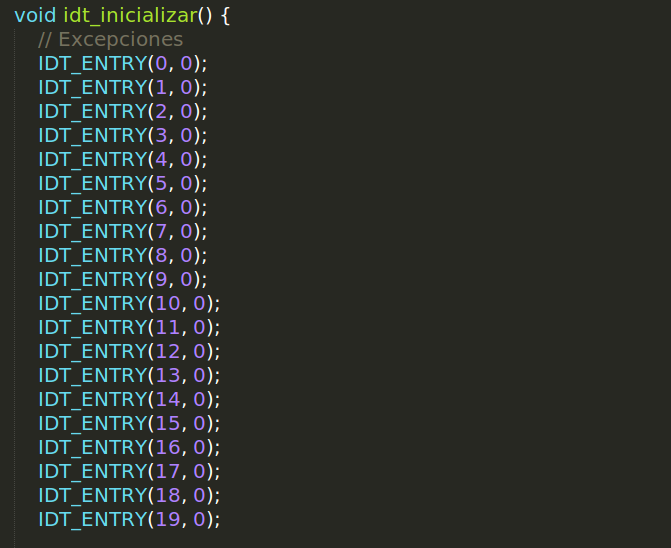
\includegraphics[width=\linewidth]{ejercicio2/idt.png}
  \caption{{\small Formato de los atributos de una interrupcion} }
\endminipage
\end{center}
\end{figure}
 \subsubsection{{\large \textit{Isr.h:}}}

 En este archivo tuvimos que declarar las siguientes funciones:
  \begin{figure}[H]
\begin{center}
\minipage{0.8\textwidth}
  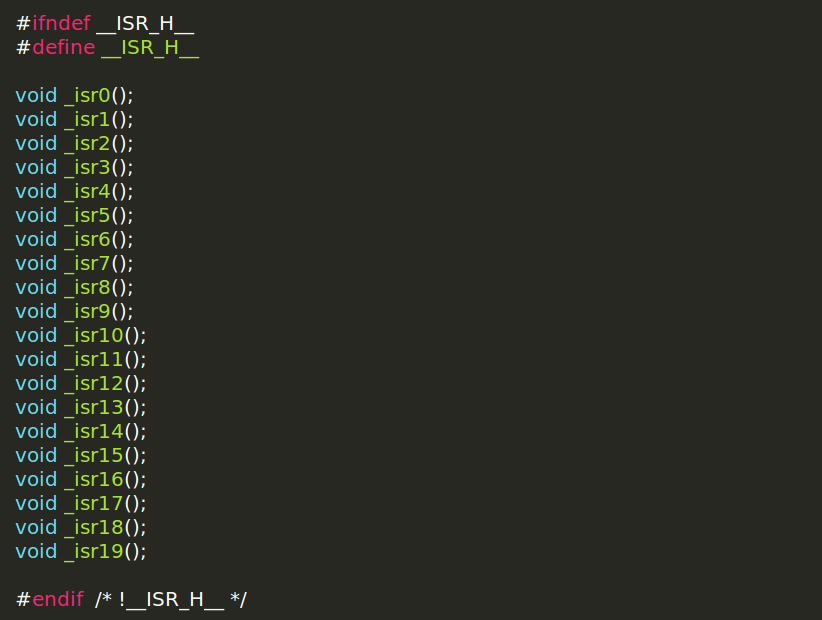
\includegraphics[width=\linewidth]{ejercicio2/isrh.png}
  \caption{{\small Formato de los atributos de una interrupcion} }
\endminipage
\end{center}
\end{figure}


 Sino, la función del archivo anterior, \textit{IDT\_ENTRY}, no compilaba, pues no las encontraba. No es necesario que estas funciones hagan algo, ya que en realidad \textit{IDT\_ENTRY} las utilizaba como macro.

 \subsubsection{{\large \textit{Isr.asm:}}}

Por último, en este archivo, atendemos las interrupciones con sus correspondientes rutinas, como en el enunciado solo se pide que se interrumpa la ejecucion del programa y se muestre por pantalla la iterrupcion que genero el problema, solamente utilizamos una funcion macro dada por la catedra que simplemente muestra dicho mensaje y ejecuta un loop infinito.\\

La macro es la siguiente:
  \begin{figure}[H]
\begin{center}
\minipage{0.6\textwidth}
  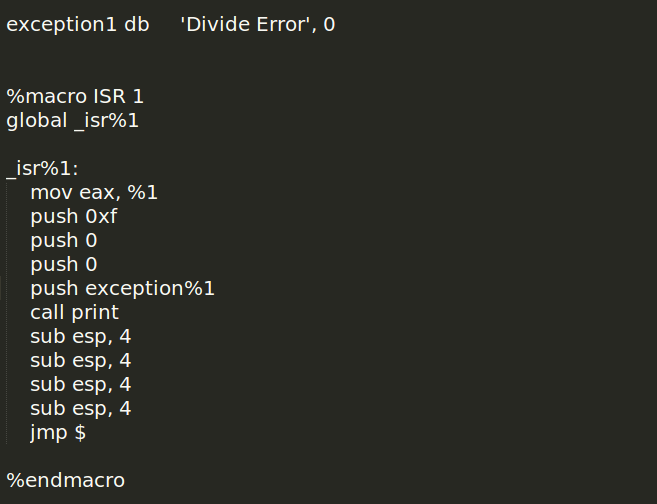
\includegraphics[width=\linewidth]{ejercicio2/macro.png}
  \caption{{\small Macro para atender interrupciones} }
\endminipage
\end{center}
\end{figure}

La macro de la imágen anterior reemplaza  \%1 por el primer parametro que recibe. Este parametro es el número correpsondiente a la interrupción, por ende cuando llegue la interrupucion $"x"$, se pushea el mensaje exception$"x"$ y print muestra por pantalla el mensaje correspondiente a la etiqueta exception$"x"$, para luego quedarse saltando infinitamente y por lo tanto interrupiendo la ejecucion del programa. En la imagen se muestra un ejemplo del mensaje que se mostraria si se produjera la interrupcion 1 , correspondiente a la division por cero.\\

Por ultimo escribimos la rutina de atencion de interrupciones, la cual simplemente llama a la macro anterior, tomando como parámetro el número de la interrupcion.

  \begin{figure}[H]
\begin{center}
\minipage{0.4\textwidth}
  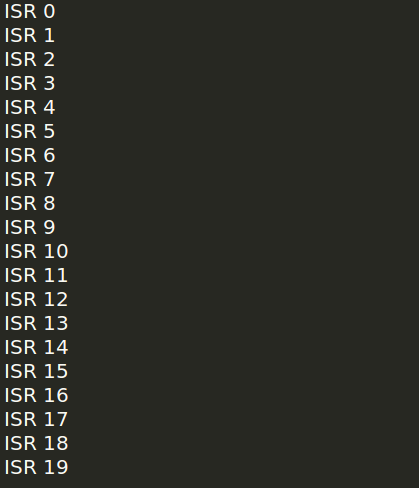
\includegraphics[width=\linewidth]{ejercicio2/israsm.png}
  \caption{{\small Rutina de atencion de interrrupciones.} }
\endminipage
\end{center}
\end{figure}


\subsection{Ítem b): Cargar y probar \textit{IDT}}

Para cargar la \textit{IDT} y probarla, agregamos las siguientes lineas al \textit{kernel}:

\begin{center}
    lidt [IDT\_DESC]\\
    mov eax, 0  $~~~~~~~$  \\
    mov ecx, 1 $~~~~~~~$    \\
    div ecx$~~~~~~~~~~~~~$
\end{center}

Obteniendo el resultado esperado:

  \begin{figure}[H]
\begin{center}
\minipage{0.8\textwidth}
  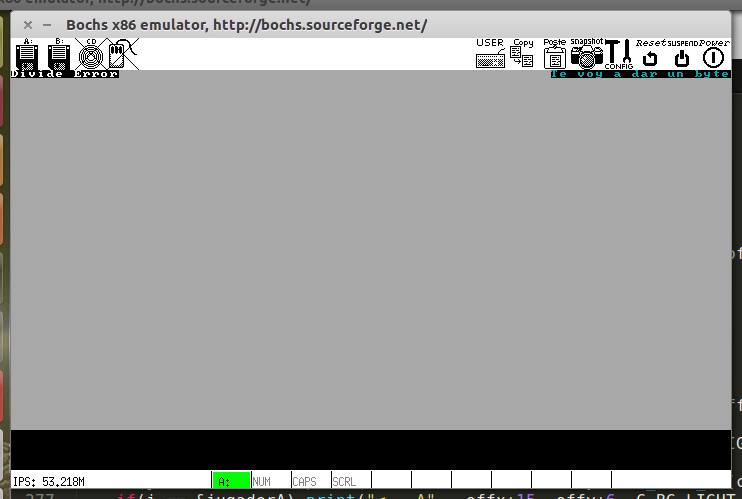
\includegraphics[width=\linewidth]{ejercicio2/division.jpg}
  \caption{{\small Rutina de atencion de interrrupciones.} }
\endminipage
\end{center}
\end{figure}



\newpage
\section{Ejercicio 3:}
\subsection{Introducción:}

En el siguiente ejercicio activaremos la páginacion básica. Completaremos el archivo \textit{mmu.c} para relizar los siguientes ítems.
\begin{itemize}
\item [\textit{a)}] Limpiar el buffer de video y pintar el mapa.
\item [\textit{b)}] Completar la función \textit{mmu\_mapear\_página(unsigned int virtual, unsigned int cr3, unsigned int física)}
\item [\textit{c)}] Utilizando la función anterior, completar la función \textit{mmu\_inicializar\_dir\_kernel} generar un directorio de páginas que mapee, usando identity mapping, las direcciones 0x00000000 a 0x003FFFFF. El directorio de páginas a inicializar se encuentra en la dirección 0x27000.
\item [\textit{d)}] Activar la paginación y verificar que el sistema sigue funcionando imprimiendo el nombre del grupo.
\item [\textit{e)}] Completar la función \textit{mmu\_unmapear\_pagina(unsigned int virtual, unsigned int cr3)}
\item [\textit{f)}] Probar la función anterior desmapeando la última página del kernel (0x3FF000).
\end{itemize}

\subsection{Ítem a): Limpiar el buffer de video y pintar el mapa \textit{IDT}}

Este ítem ya lo implementamos anteriormente, el mapa ya se encuentra pintado. Lo hicimos en el ejercicio 2, al utilizar las funciones  \textit{aux\_limpiarPantalla} y \textit{screen\_inicializar}. \\

\subsection{Ítem b): Completar la función \textit{mmu\_mapear\_página(unsigned int virtual, unsigned int cr3, unsigned int física)}}

En este punto realizamos la siguiente función: 

\begin{figure}[H]
\begin{center}
\minipage{1.0\textwidth}
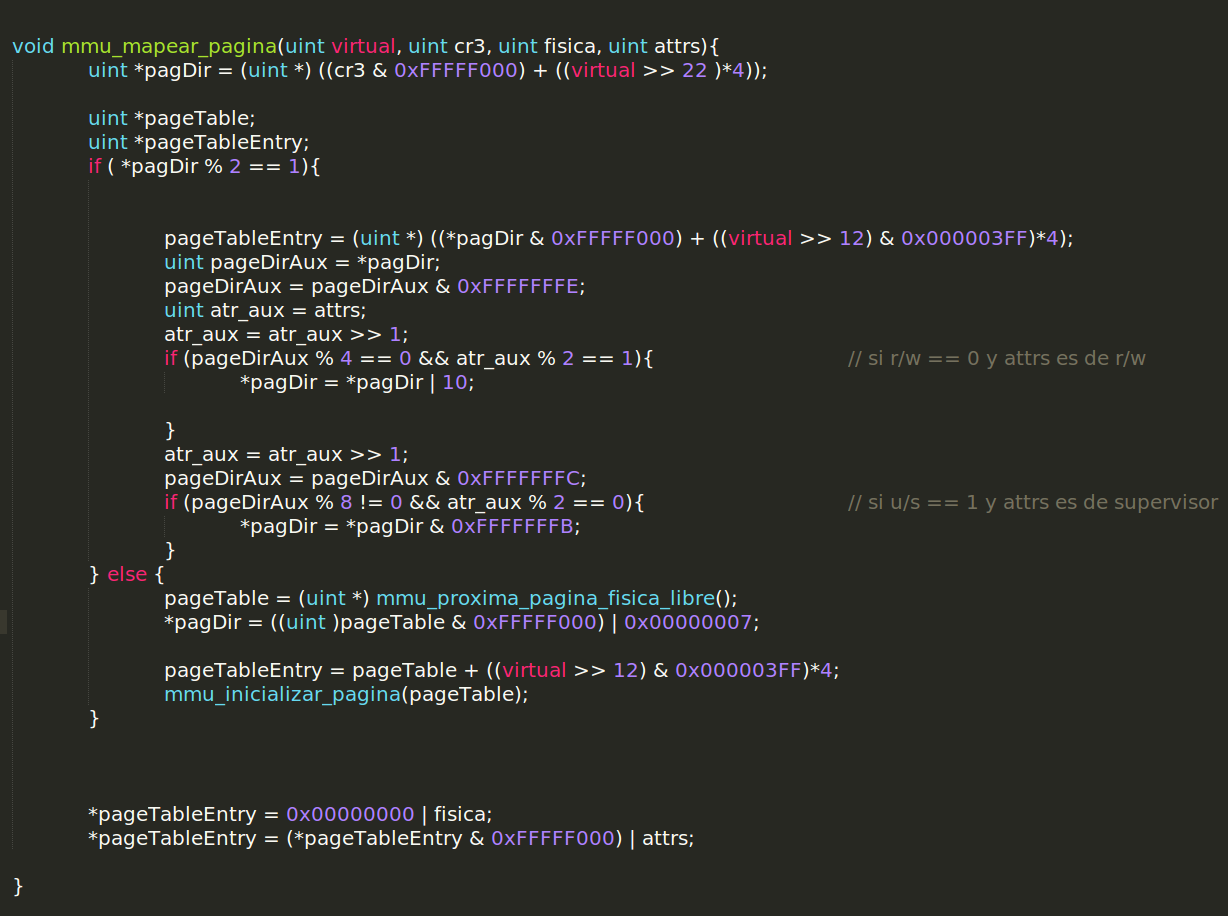
\includegraphics[width=\linewidth]{ejercicio3/mappag.png}
\caption{{\small Función mapeadora} }
\endminipage
\end{center}
\end{figure}

Lo que realiza esta función es lo siguiente: 

\begin{itemize}
	\item[A:] Recibe como parámetro una dirección virtual, una física, un \textit{CR3} y la informacion sobre los atributos. 

	\item[B:] Como \textit{CR3} tiene la siguiente forma:
	 
	 \begin{figure}[H]
	 \begin{center}
	 \minipage{0.6\textwidth}
  	 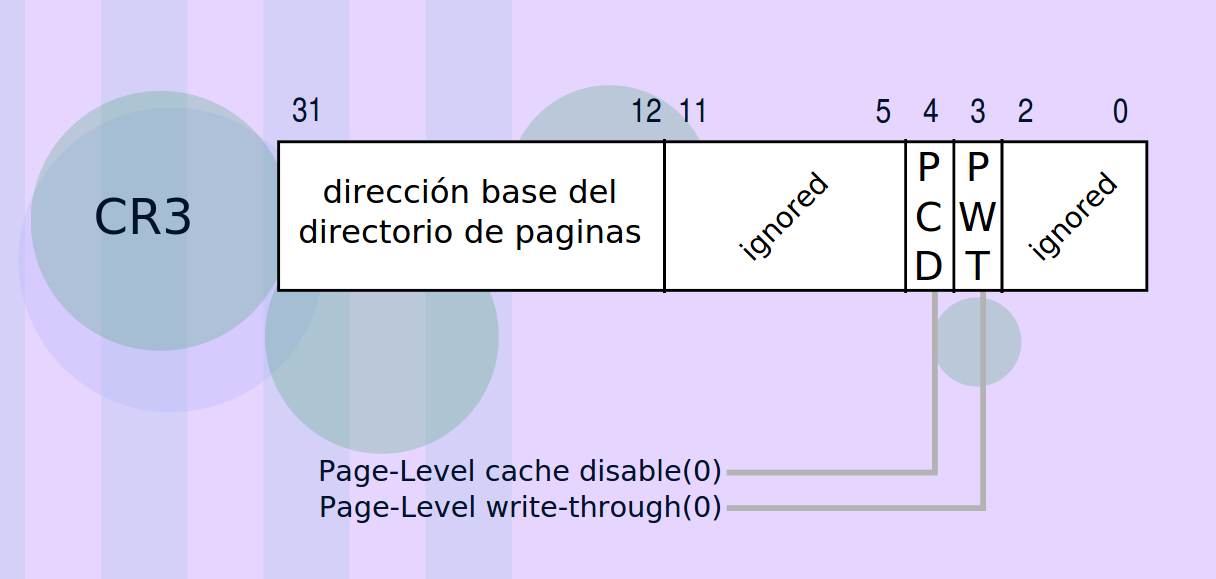
\includegraphics[width=\linewidth]{ejercicio3/cr3.png}
  	 \caption{{\small Formato \textit{CR3} }}
	 \endminipage
	 \end{center}
	 \end{figure}

	  Le hacemos un and lógico con 0xFFFFF000, de esta forma nos quedamos solo con la direccion base del directorio de páginas del cr3. Luego shifteamos la direccion virtual del parámetro de entrada en 22 posiciones, para quedarnos con el offset de la misma y multiplicamos este offset por 4 pues los punteros de las páginas de directorio ocupan 32 bytes y cada posicion de memoria es de 8.\\

	  Ahora sumamos la direccion base del directorio de páginas con el offset anterior y obtenemos la dirección de la tabla de página que buscabamos.

	 \begin{figure}[H]
	 \begin{center}
	 \minipage{0.8\textwidth}
  	 
\includegraphics[width=\linewidth]{ejercicio3/fun1.png}
  	 \caption{{\small Formato \textit{CR3} }}
	 \endminipage
	 \end{center}
	 \end{figure}

	 \item[C:] Lo siguiente es fijarse si la direcion de la tabla de página obtenida existe o no. Para esto nos fijamos que en modulo 2 la direccion anterioirmente obtenida. Asi obtenemos el útlimo bit de la misma, si es 1 (P) sabemos que esta presente y si es 0 sabemos que no lo esta ($\neg$P) y tenemos que crearla
	 \begin{itemize}
	  \item[P: ] Si esta presente, tenemos que encontrar la posición de la tabla de página deseada. Para eso, realizamos un and lógico con la dirección obtenida anteriormente y  0xFFFFF000 para obtener la direccion base de la tabla de página (en la cual buscaremos la posicion deseada).

	 \begin{figure}[H]
	 \begin{center}
	 \minipage{0.6\textwidth}
  	 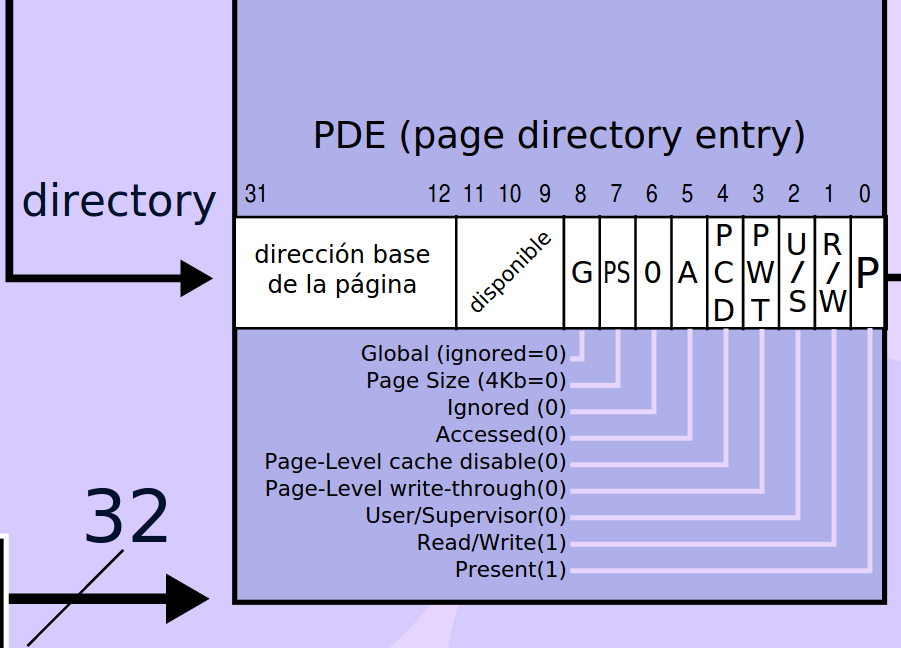
\includegraphics[width=\linewidth]{ejercicio3/fun2.png}
  	 \caption{{\small Formato de una posicion del directorio de tabla de páginas}}
	 \endminipage
	 \end{center}
	 \end{figure}

	  Luego shiftemos 12 posiciones la direccion vitual del parámetro de entrada para obtener el segundo offset necesesario y le hacemos un and lógico con 0x000003FF ara que solo quede la informacion que queremos y limpiar la posible basura que haya. \\

	  Este offset lo multiplicamos por 4 por la misma razón explicada anteriormente y se lo sumamos a la direccion base obtenida antes. Asi obtenemos la posicion de la tabla de página deseada.\\

	  En este caso, es necesario checkear si los atributos que se encuentran en la posicion recientemente encontrada son los mismos que los que se encontraban en la posicion del directorio de páginas encontrada en B. Obtenemos los atributos, y los comparamos, y en caso de ser necesario los cambiamos. \\

	  \begin{figure}[H]
	  \begin{center}
	  \minipage{0.6\textwidth}
  	  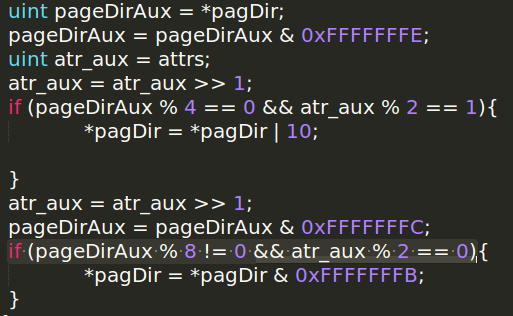
\includegraphics[width=\linewidth]{ejercicio3/fun3.png}
  	  \caption{{\small Comparacion y cambio de atributos}}
	  \endminipage
	  \end{center}
	  \end{figure}


	  \item[$\neg$P: ] Si la página no estaba presente, en necesario crearla. Entonces pedimos una dirección para crearla con la función \textit{mmu\_proxima\_página\_fisica\_libre()}. Luego ponemos esta direccion obtenida en el directorio de tabla de páginas, en la posicion obtenida en B, con los atributos correspondientes (para eso el or lógico con 0x00000007 )\\

	  \begin{figure}[H]
	  \begin{center}
	  \minipage{0.5\textwidth}
  	  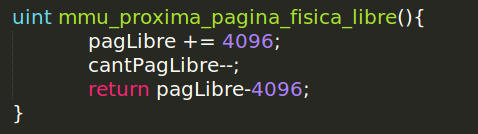
\includegraphics[width=\linewidth]{ejercicio3/proxpaglibre.png}
  	  \caption{{\small Función que nos da una posicion libre para poner una página. La variable pagLibre es una variable global inicializada con el valor 0x100000, y cantPaglibre en 768}}
	  \endminipage
	  \end{center}
	  \end{figure}

	  Por último obtenemos la posicion deseada de la tabla de página obtenida en B de la misma manera que cuando la página esta presente e incicializamos la tabla de página llenandola de ceros.

	   \begin{figure}[H]
	  \begin{center}
	  \minipage{0.5\textwidth}
  	  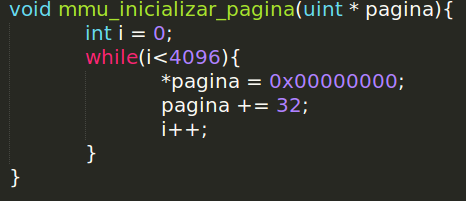
\includegraphics[width=\linewidth]{ejercicio3/inicializarpag.png}
  	  \caption{{\small Función que inicializa una página}}
	  \endminipage
	  \end{center}
	  \end{figure}

	 \end{itemize}

	 \item[D:] Ahora que tenemos todo en orden y la posición de la tabla de página deseada, procedemos a poner en esta posición la direccion física pasada por parámetro con los atributos tambien pasados por parámetro.

	  \begin{figure}[H]
	  \begin{center}
	  \minipage{0.6\textwidth}
  	  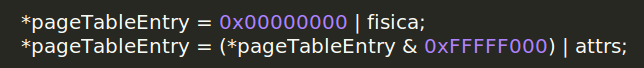
\includegraphics[width=\linewidth]{ejercicio3/fun4.png}
  	  \caption{{\small Identity mapping}}
	  \endminipage
	  \end{center}
	  \end{figure}

	  Como es Identity Mapping alcanza con poner en esta posición el resultado de hacer un or lógico con la direccion física y luego un or lógico con los atributos.

\end{itemize}
	  
	  \subsection{Ítem c): Inicializar el directorio de páginas en 0x00027000  y mapear las direcciones desde la 0 hasta la 0x003FFFFF con Identity Mapping\textit{IDT}}

	  Para realizar lo pedido completamos la funcion \textit{mmu\_inicializar\_dir\_kernel} mostrada a continuación:

	  \begin{figure}[H]
	  \begin{center}
	  \minipage{0.7\textwidth}
  	  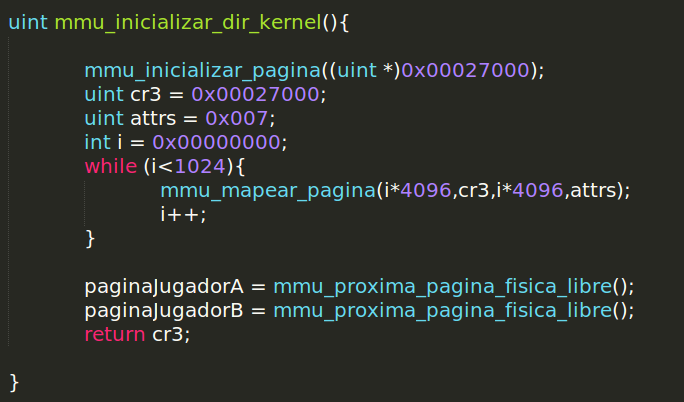
\includegraphics[width=\linewidth]{ejercicio3/inikernel.png}
  	  \caption{{\small }}
	  \endminipage
	  \end{center}
	  \end{figure}

	  Esta funcion comienza creando una tabla de páginas vacía en la dirección 0x27000, la cual va a actuar como directorio de páginas. Luego crea la variable \textit{Attrs} y la inicializa con el valor 0x007, el cual corresponde a los atributos que queremos que tenga el directorio de páginas, osea que P = 1, sea de lectura y escritura y sea de sistema. Tambien crea la variable \textit{Cr3} el cual se le asigna el valor  0x00027000 para que tenga la direccion base y los atributos correspondientes al directorio de paginas que queremos inicializar.\\

	 Para mapear cada posición del directorio recientemente creado se llama a la función del ítem anterior . LLamamos a esta función con las variables  \textit{Cr3} y \textit{Attrs} anteriormente creadas, y en cada iteracion se le da una posicion nueva del directorio para que haga el correpsondiente mapeo. \\

	 Por último es necesario que cada jugador tenga una página, por eso le asignamos a cada uno una página libre.

\subsection{Ítem d): Activar la paginación y verificar que el sistema sigue funcionando imprimiendo el nombre del grupo.}

	Activamos la paginacion escribiendo en el kernel las siguientes líneas:

	\begin{center}
    	$~$  \\ 	 
	Inicializar el directorio de paginas: \\
	$~$  \\ 	 
  	call mmu\_inicializar\_dir\_kernel  $~~~~~$  \\ 

  	$~$  \\ 
    	Cargar directorio de paginas:  $~~~~~~$  \\
    	$~$  \\ 

    	mov eax, 0x00027000  $~~~~~~~~~~~~~~~~~$  \\
    	mov cr3, eax  $~~~~~~~~~~~~~~~~~~~~~~~~~~~~$  \\

    	$~$  \\ 
    	Habilitar paginacion:  $~~~~~~~~~~~~~~~~$  \\
       	$~$  \\ 
   
        	mov eax, cr0  $~~~~~~~~~~~~~~~~~~~~~~~~~~~~$  \\
    	or eax, 0x80000000  $~~~~~~~~~~~~~~~~~~~$  \\
    	mov cr0, eax  $~~~~~~~~~~~~~~~~~~~~~~~~~~~~$  \\

	\end{center}

	Luego verificamos que el sistema sigue funcionando imprimiendo por pantalla el nombre del grupo

	  \begin{figure}[H]
	  \begin{center}
	  \minipage{0.9\textwidth}
  	  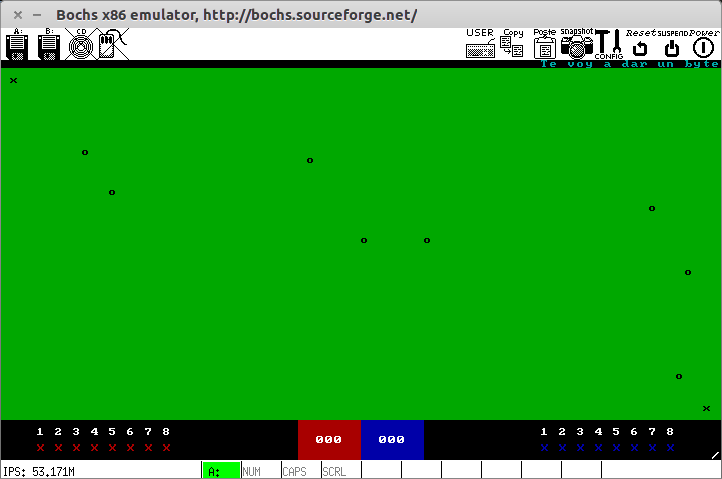
\includegraphics[width=\linewidth]{ejercicio3/nombre.png}
  	  \caption{{\small }}
	  \endminipage
	  \end{center}
	  \end{figure}

\subsection{Ítem e): Completar la función \textit{mmu\_unmapear\_pagina(unsigned int virtual, unsigned int cr3)}}

	Para unmapear una dirección virtual realizamos la siguiente función 

	  \begin{figure}[H]
	  \begin{center}
	  \minipage{0.9\textwidth}
  	  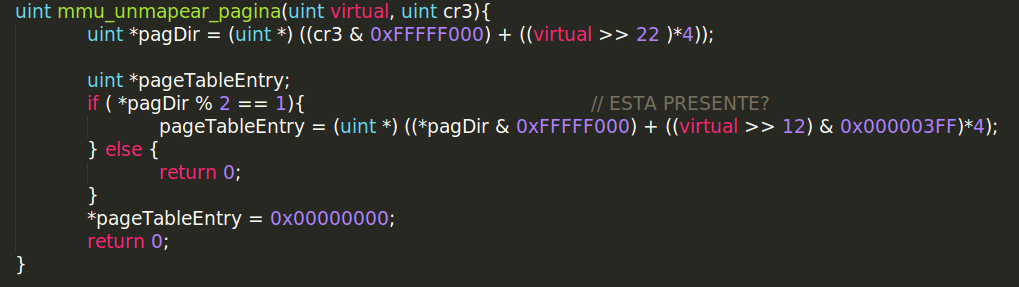
\includegraphics[width=\linewidth]{ejercicio3/unmap.png}
  	  \caption{{\small Identity mapping}}
	  \endminipage
	  \end{center}
	  \end{figure}

	La cual realiza el mismo cálculo que en el ítem 2 para acceder a la posicion de tabla de pagina buscada en el directorio de páginas y luego si esta pagina esta presente se hace un calculo tambien explicado anteriormente para acceder a la posicion deseada en esta pagina. Una vez obtenida esta posicion se procede a llenarla con ceros.


\subsection{Ítem f): Probar la función anterior desmapeando la última página del kernel (0x3FF000).} 

	 Para probar la función anterior, escribimos en el kernel las siguientes lineas:
	 \begin{center}

	 $~$  \\ 
	 Le pasamos los parametros a la funcion: \\
	 $~$  \\ 
	 mov eax, cr3 $~~~~~~~~$\\
   	 push eax$~~~~~~~~~~~~~~$ \\
   	 mov eax, 0x3FF000 \\
   	 push eax $~~~~~~~~~~~~~$\\

   	 $~$  \\ 
   	 La llamamos:\\
   	 $~$  \\ 
   	 call mmu\_unmapear\_pagina \\

   	 $~$  \\ 
   	 Limpiamos pila:\\
             $~$  \\ 
  	 pop eax \\
  	 pop eax \\
	 \end{center}

	 De esta manera llamamos a la función, y para ver que los resultados son los deseados, usamos el comando \textit{Info tab} de \textit{bochs} para ver hasta donde llega el mapeo de paginas y obetemos que llega hasta la direccion 0x3FEFFF en vez de llegar hasta 0x3FEFFF, por lo tanto podemos decir que la función hizo lo devido.
 
	  \begin{figure}[H]
	  \begin{center}
	  \minipage{0.9\textwidth}
  	  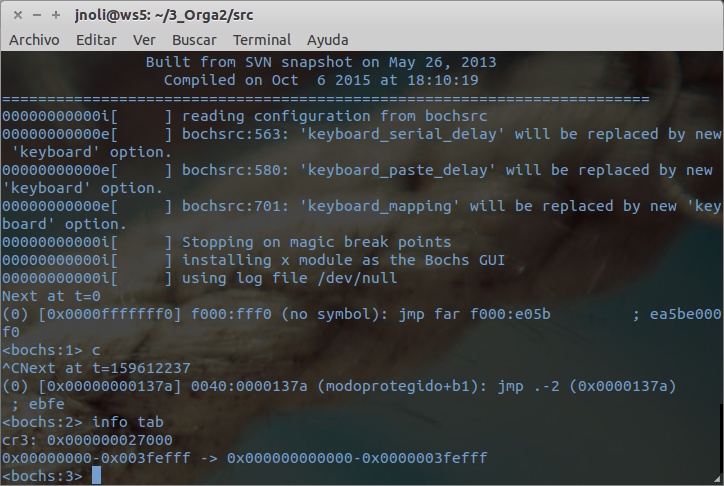
\includegraphics[width=\linewidth]{ejercicio3/unmaproof.png}
  	  \caption{{\small Identity mapping}}
	  \endminipage
	  \end{center}
	  \end{figure}
	






\newpage
\section{Ejercicio 4:}
\subsection{Introducción:}

\begin{itemize}
\item [\textit{a)}] Completar \textit{inicializar\_mmu} que se encargue de inicializar las estructuras globales necesarias para administrar la memoria en el área libre (un contador de páginas libres).
\item [\textit{b)}] Completar la función \textit{mmu\_inicializar\_memoria\_perro}.
\end{itemize}

\subsection{Ítem a): Completar \textit{inicializar\_mmu}.}

	Para realizar esta función simplemente creamos en el archivo \textit{mmu.c} las variables globales las cuales puden ser usadas por el resto de las funciones:	

	$~$

	uint pagLibre = 0x100000 

	uint cantPagLibre = 768 

	uint paginaJugadorA

	uint paginaJugadorB\\

\subsection{Ítem b): Completar la función \textit{mmu\_inicializar\_memoria\_perro}.}

La función la realizamos de la siguiente manera:

\begin{figure}[H]
\begin{center}
\minipage{1.05\textwidth}
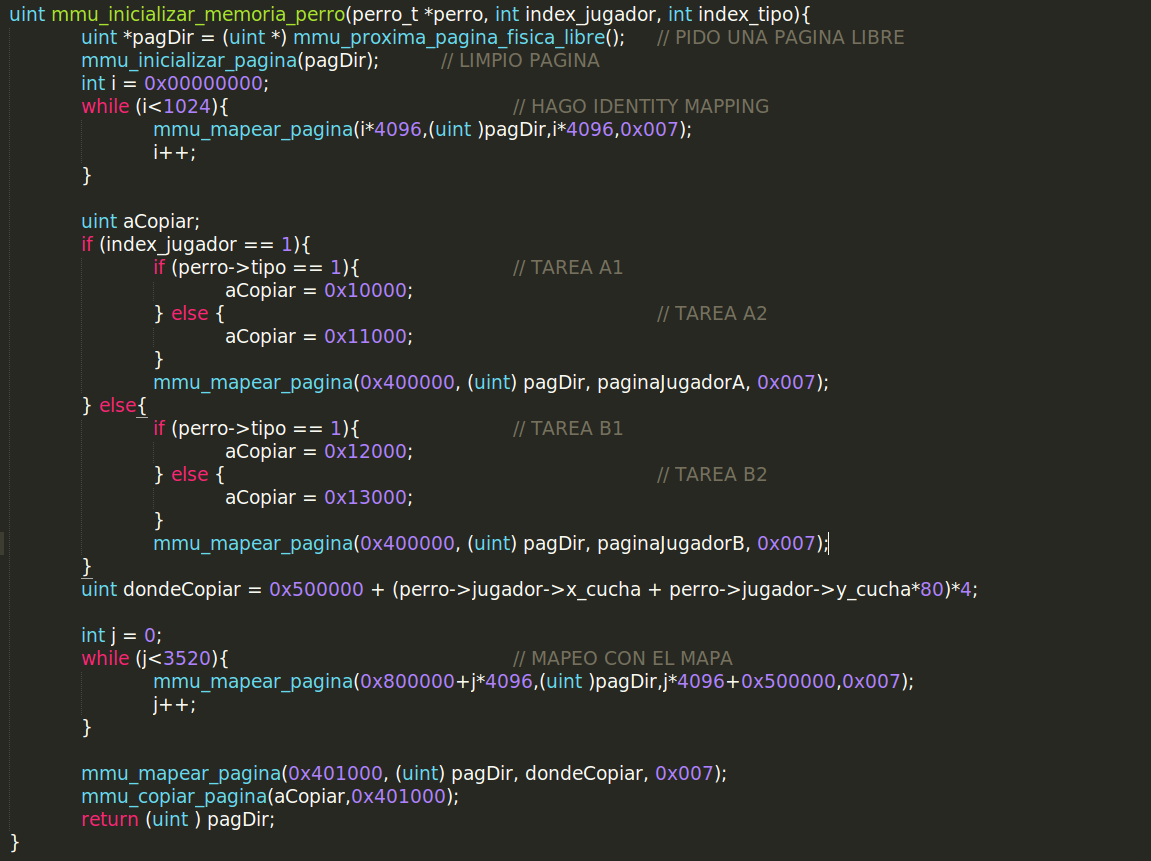
\includegraphics[width=\linewidth]{ejercicio4/funprin.png}
\caption{{\small Función principal} }
\endminipage
\end{center}
\end{figure}


La función realiza lo siguiente: 

\begin{itemize}

	\item[A:] Recibe como parametros un perro, un int que sirve para indicar que jugador es y otro int para identificar el tipo de perro.

	\item[B:] Comienza pidiendo un lugar para crear una página libre, para eso llama a la función \textit{mmu\_proxima\_pagina\_fisica\_libre()}. Una vez obtenida la posicion, procede a crear la pagina y luego la mapea con la funcion \textit{mmu\_mapear\_pagina}

	\begin{figure}[H]
	\begin{center}
	\minipage{0.65\textwidth}
	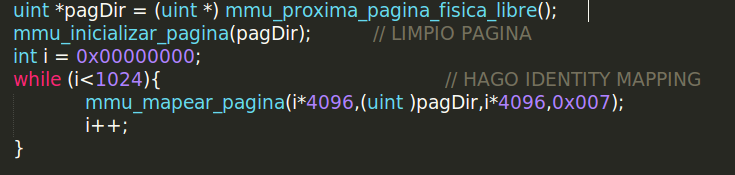
\includegraphics[width=\linewidth]{ejercicio4/fun1}
	\caption{{\small } }
	\endminipage
	\end{center}
	\end{figure}

	\item[C:]  Luego, para saber que tarea copiar identifica que jugador es, usando el parámetro de entrada \textit{index\_jugador}, luego identifica que tipo de perro es , usando la variable de entrada \textit{index\_tipo}. Con esa informacion, la función sabe donde esta la tarea que tiene que copiar. Ademá es necesario que se le mapee esta nueva tarea al jugador correspondiente por eso, dependiendo de que jugador sea, se le mapea esta nueva tarea.
	 
	\begin{figure}[H]
	\begin{center}
	\minipage{0.7\textwidth}
	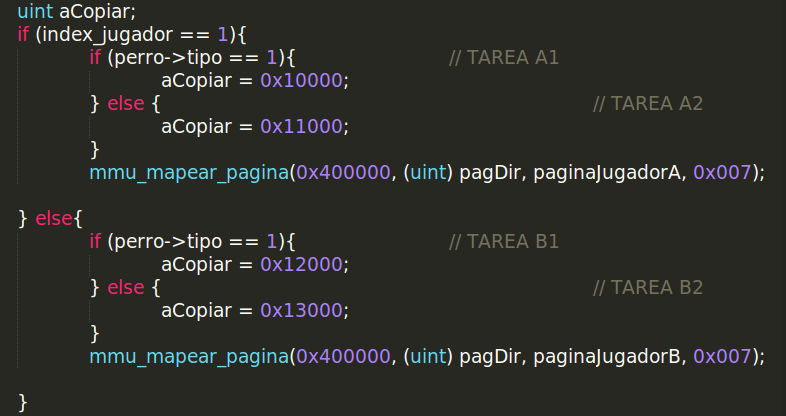
\includegraphics[width=\linewidth]{ejercicio4/fun2}
	\caption{{\small } }
	\endminipage
	\end{center}
	\end{figure}

	\item[D:] Después de mapear el mapa devuelta es necesario mapear la dirección 0X401000 con la posición donde tiene que estar la tarea. Para saber en que dirección tiene que estar la tarea (o sea dónde va a estar el perro), la función toma la posición 0x500000 (posición donde se encuentra el mapa) y le suma el valor X y el valor Y de la cucha del perro y mapea 0X401000 con la dirección obtenida. De esta manera el kernel sabe donde deben estar los perros y finalmente se puede copiar la tarea a la dirección 0X401000, la cual va a estar mapeada correctamente al lugar donde hay que poner a los nuevos perros/tareas.
	
\end{itemize}

\newpage
\section{Ejercicio 5:}
\subsection{Introducción:}

En este ejercicio nos encargaremos del manejo de las interrupcíones del reloj, teclado y otra interrupcíon de software 0x46. Se pide:

\begin{itemize}
\item [\textit{a)}] Completar las entradas necesarias en la \textit{IDT}.
\item [\textit{b)}] Escribir la rutina asociada a la interrupcíon de reloj, de manera que por cada tick, se muestre la animacion de un cursor rotando
\item [\textit{c)}]  Escribir la rutina asociada a la interrupcíon de teclado, para aquellas teclas a utilizar en el juego, para que se imprima la misma en la pantalla
\item [\textit{d)}] Escribir la rutina asociada a la interrupcíon de software 0x46 para que modifique el valor de \textit{eax} por 0x42
\end{itemize}



\subsection{Ítem a): Completar la \textit{IDT}}

Comenzamos agregando las interrupcíones a la \textit{IDT}. Utilizamos para el reloj y el teclado las posiciones 32 y 33 respectivamente, pues son las primeras disponibles no utilizadas por el procesador. Para la interrupcíon por software, utilizamos la posicion 70, pues esta se llamara al llamar a int 0x46 $=$ 70. Las declaramos con privilegio 0, pues son de sistema y no se querria que algo externo al sistema los controle. \\
Para esto utilizamos la macro anteriormente explicada, con los siguientes parametros:

\begin{figure}[H]
\begin{center}
\minipage{0.25\textwidth}
  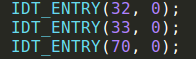
\includegraphics[width=\linewidth]{ejercicio5/idt.png}
\endminipage
\end{center}
\end{figure}

Además, las definimos en \textit{isr.h}, para luego escribir su rutina.

\begin{figure}[H]
\begin{center}
\minipage{0.25\textwidth}
  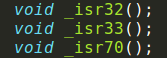
\includegraphics[width=\linewidth]{ejercicio5/isr.png}
\endminipage
\end{center}
\end{figure}

\subsection{Ítem b): Rutina del reloj}

El código es el siguiente:
\begin{figure}[H]
\begin{center}
\minipage{0.5\textwidth}
  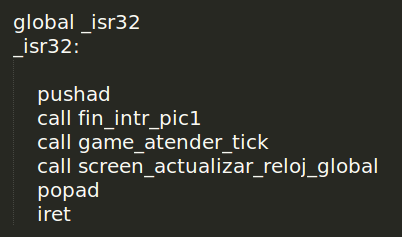
\includegraphics[width=\linewidth]{ejercicio5/rutinaReloj.png}
\endminipage
\end{center}
\end{figure}

Cada vez que se llame, la interrupcíon hara lo siguiente. Pusheara todos los registros de proposito general (lo cual en realidad no es necesario, dado que la interrupcíon no los modifica). Llamara a la fnción \textit{fin$\_$intr$\_$pic1} para decir al pic que la interrupcíon fue atendida. Luego llamara a las fnciónes \textit{game$\_$atender$\_$tick }y \textit{screen$\_$actualizar$\_$reloj$\_$global} para mostrar la animacion por pantalla. Luego popeara los registros y volvera de la interrupcíon con la instruccion iret


\subsection{Ítem c): Rutina del teclado}

El código es el siguiente:
\begin{figure}[H]
\begin{center}
\minipage{0.35\textwidth}
  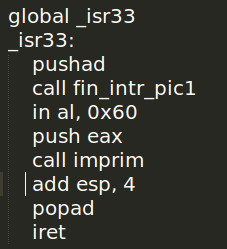
\includegraphics[width=\linewidth]{ejercicio5/rutinaTeclado.png}
\endminipage
\end{center}
\end{figure}

Igual que la interrupcíon anterior, comienza pusheando todos los registros. En este caso, es necesario preservar \textit{eax}, pues lo modificamos. Nuevamente llamamos a \textit{fin$\_$intr$\_$pic1}. Luego utilizamos la operacion \textit{in}, para mover al registro al el 
Leemos del teclado a traves del puerto 0x60 y obtenemos el scan code en \textit{eax}. Pusheamos este valor y llamamos a la función \textit{imprim} creada por nosotros. Esta fnción se encarga de traducir el scan code en una letra (en caso de que sea válido) y luego llama a la función print para mostrarlo por pantalla. Finalmente restauramos la pila, popeamos los registros y volvemos de la interrupcíon.

\subsection{Ítem d): Rutina 0x46}


El código es el siguiente:

\begin{figure}[H]
\begin{center}
\minipage{0.3\textwidth}
  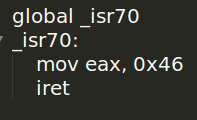
\includegraphics[width=\linewidth]{ejercicio5/rutina0x46.png}
\endminipage
\end{center}
\end{figure}

Lo único que hace esta interrupción es modificar el registro \textit{eax}. Por lo tanto no es necesario salvar los registros. Esta interrupción sera modificada mas adelante

\newpage
\section{Ejercicio 6:}
\subsection{Introducción:}

En este ejercicio trabajaremos con todo lo relacionado a la \textit{TSS}, realizaremos los siguientes ítems:

\begin{itemize}



\item [\textit{a)}]  Definir las entradas en la \textit{GDT} que considere necesarias para ser usadas como descriptores de \textit{TSS}.

\item [\textit{b)}] Completar la entrada de la \textit{TSS} de la tarea Idle con la información de la tarea Idle. La tarea Idle se encuentra en la dirección 0x00016000. La pila se alojará en la misma dirección que la pila del kernel y debe compartir el mismo CR3 que el kernel.

\item [\textit{c)}]  Construir una función que complete una TSS libre con los datos correspondientes. El código de las tareas se encuentra a partir de la dirección 0x00010000. Para la dirección de la pila se debe utilizar el mismo espacio de la tarea, la misma crecerá desde la base de la tarea. Para el mapa de memoria se debe construir uno nuevo utilizando la función \textit{mmu\_inicializar\_dir\_perro}. Además, tener en cuenta que cada tarea utilizará una pila distinta de nivel 0. 

\item [\textit{d)}] Completar la entrada de la \textit{GDT} correspondiente a la tarea\_inicial.

\item [\textit{e)}]  Completar la entrada de la \textit{GDT} correspondiente a la tarea Idle.

\item [\textit{f)}]  Escribir el código necesario para ejecutar la tarea Idle, es decir, saltar intercambiando las TSS, entre la tarea\_inicial y la tarea Idle.

\item [\textit{g)}] Modificar la rutina de la interrupción 0x46, para que implemente los servicios según se indica en la sección 4.4, sin desalojar a la tarea que realiza el syscall.

\item [\textit{h)}]  Ejecutar una tarea perro manualmente. Es decir, crearla y saltar a la entrada en la \textit{GDT} de su respectiva TSS.

\end{itemize}

\subsection{Item a) Definir entradas de la \textit{GDT} necesarias}
Para este punto definimos 18 nuevas entradas en la \textit{GDT}.\\

Las primeras dos nuevas entradas de la \textit{GDT} corresponden a la \textit{Tarea inicial} y a la tarea \textit{idle} respectivamente. 

\begin{figure}[H]
\begin{center}
\minipage{0.80\textwidth}
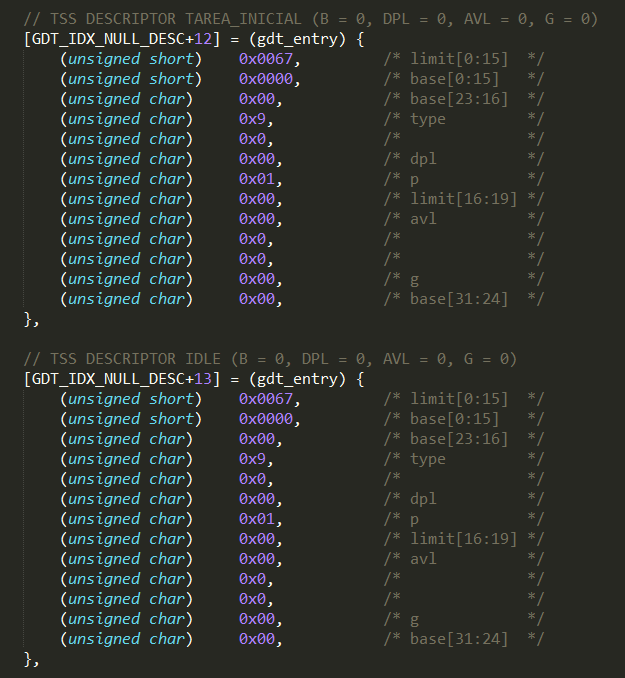
\includegraphics[width=\linewidth]{ejercicio6/gdt_inicial_idle.png}
\caption{{\small \textit{Entrada de la \textit{GDT} correspondiente a la tarea inicial y a la idle }}}
\endminipage
\end{center}
\end{figure}

Las siguientes 8 entradas corresponden a los 8 perros del \textbf{jugador A} ordenadas en orden decreciente en el número de perros, es decir, el \textit{id} y finalmente las últimas 8 entradas corresponden a los 8 perros del \textbf{jugador B } también ordenadas decrecientemente por \textit{id}.\\

\begin{figure}[H]
\begin{center}
\minipage{0.80\textwidth}
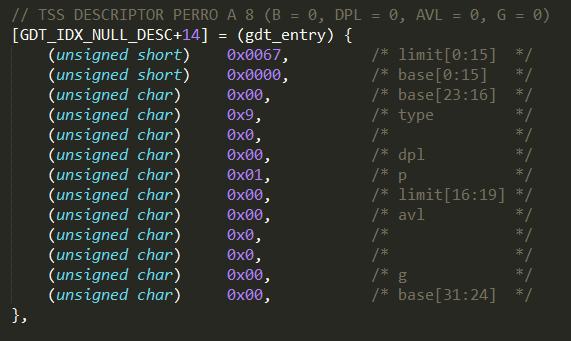
\includegraphics[width=\linewidth]{ejercicio6/gdt_perro.png}
\caption{{\small \textit{Entrada de la \textit{GDT} correspondiente al descriptor de tss de la tarea perro }}}
\endminipage
\end{center}
\end{figure}


\subsection{Item b)}
Para este item hacemos lo siguiente, primero completamos el campo \textit{base} de la entrada de la \textit{GDT} correspondiente a la tarea \textit{idle}.Para ello le asignamos la dirección 0x00016000 tal como indica el enunciado.\\
Como también nos dicen que comparte el \textit{esp} con el \textit{kernel} entonces en la entrada \textit{esp} de la \textit{TSS} le asignamos 0x27000 que era el \textit{esp} asignado al kernel.Además como comparten el \textit{cr3} le asigno a la entrada correspondiente en la \textit{TSS} 0x28000.\\% por qué? ni idea
La siguiente imagen muestra como queda completo el descriptor de la \textit{TSS}\\

\begin{figure}[H]
\begin{center}
\minipage{0.80\textwidth}
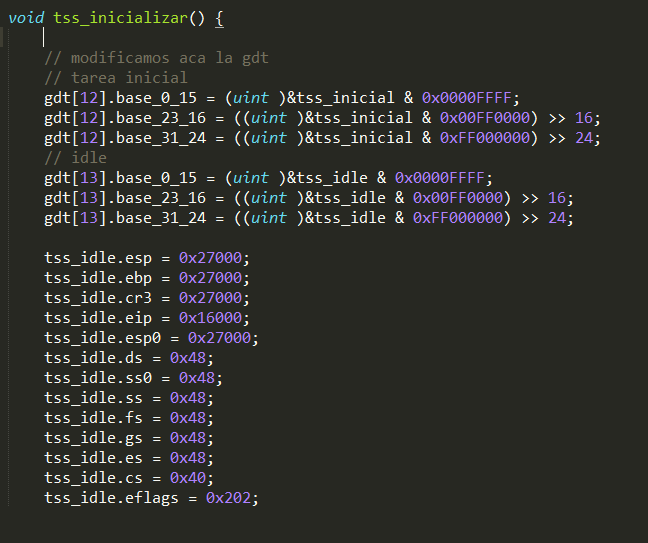
\includegraphics[width=\linewidth]{ejercicio6/tss_iddle_inicial.png}
\caption{{\small \textit{ Completamos el desscriptor de la\textit{TSS} correspondiente a la tarea iddle y a la inicial}}}
\endminipage
\end{center}
\end{figure}



\subsection{item c)}
Lo que nos piden en este punto es hacer la función $void$ $tss\_completar(int$ $jugador, int$ $perro, perro\_t *perro)$\\
Lo primero que  hacemos en esta función es pedir una nueva página libre para usarla como una pila de nivel 0 para la tarea.\\
Lo siguiente es preguntar si es la tarea (el perro) es una tarea correspondiente al \textbf{jugador A} o al \textbf{jugador B}. Para saber donde guardar el descriptor. Para cada perro de ambos jugadores se realiza lo siguiente:
\begin{itemize}

\item En los campos \textit{cs}, \textit{es}, \textit{gs}, \text{ss}, \textit{ds}, \textit{fs} tienen los segmentos definidos anteriormente en la \textit{GDT}.\\
\item La entrada \textit{esp} tiene 0x0402000-12.\\
\item La entrada \textit{eip} tiene 0x00401000.\\
\item La entrada \textit{eflags} = 0x202.\\
\item La entrada \textit{esp0} = Es la posicion de la página libre pedida mas 4kb pues tiene apilado en la pila los argumentos.\\
\item La entrada \textit{iomap} = 0xFFFF.\\
\item La entrada \textit{ss0} = 0x48.\\
\item El nuevo \textit{cr3} va a ser el devuelto por la función \textit{mmu\_inicializar\_memoria\_perro}. Asignamos el \textit{cr3}  al campo correspondiente y actualizamos la entrada correspondiente a la \textit{GDT} para esa tarea seteando los campos base e índice.
\end{itemize}

La siguiente imágen muestra dicho proceso.\\

\begin{figure}[H]
\begin{center}
\minipage{0.80\textwidth}

\includegraphics[width=\linewidth]{ejercicio6/tss_perro.png}
\caption{{\small }}
\endminipage
\end{center}
\end{figure}


\subsection{item d)}

La entrada de la \textit{GDT} correspondiente a la tarea inicial en principio la definimos con cualquier valor  en la base pero con los valores correspondientes en los demás campos.

\begin{figure}[H]
\begin{center}
\minipage{1.00\textwidth}
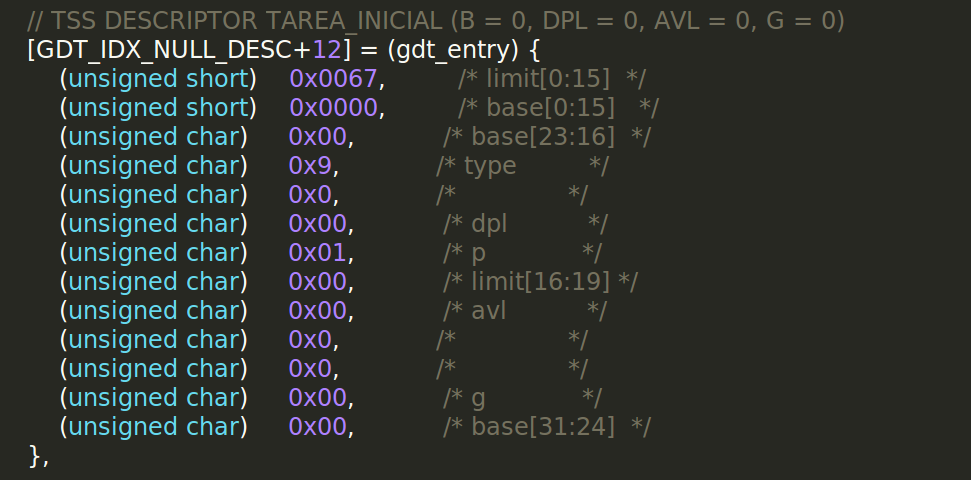
\includegraphics[width=\linewidth]{ejercicio6/gdt_tarea_inicial.png}
\caption{{\small \textit{Entrada de la \textit{GDT} correspondiente a la tarea inicial }}}
\endminipage
\end{center}
\end{figure}


Luego con la función ºtextit{tss\_inicializar()} le asignamos la base correspondiente.

\begin{figure}[H]
\begin{center}
\minipage{1.00\textwidth}
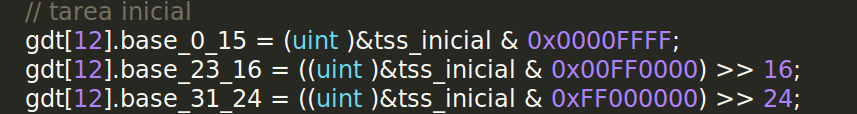
\includegraphics[width=\linewidth]{ejercicio6/tss_inicializar_base_inicial.png}
\caption{{\small \textit{Entrada de la \textit{GDT} correspondiente a la tarea inicial }}}
\endminipage
\end{center}
\end{figure}

\subsection{item e)}
Esta sección es similar a la anterior. Creamos una entrada en la \textit{GDT} para esta tarea y en la función \textit{tss\_inicializar()} seteamos los valores correspondientes para su base en la \textit{GDT} y también seteamos su TSS.\\
Como nos dicen que la tarea se encuentra en la dirección 0x00010000 ese es el valor que ponemos en la base y por el enunciado va a compartir el CR3. Lo mismo con su pila.\\

\begin{figure}[H]
\begin{center}
\minipage{1.00\textwidth}
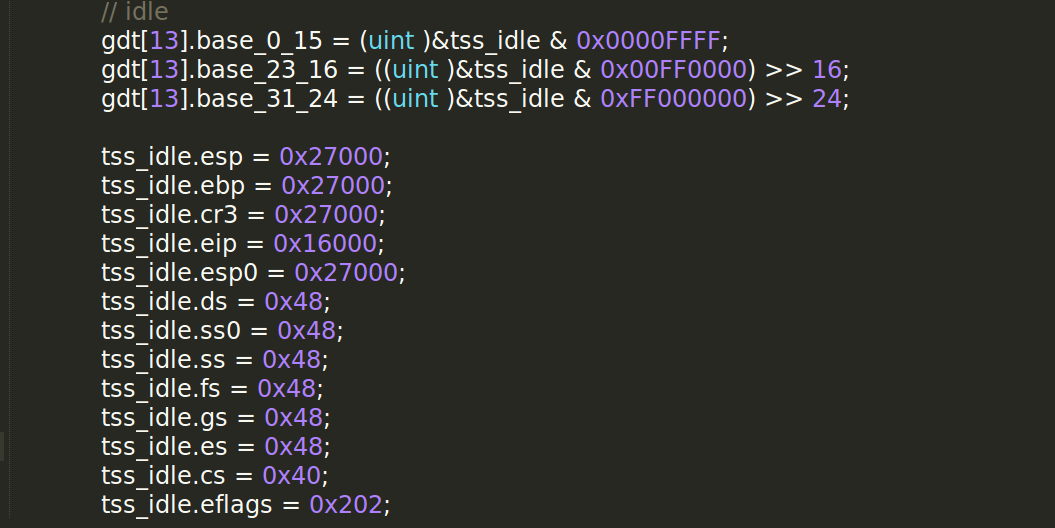
\includegraphics[width=\linewidth]{ejercicio6/tss_idle.png}
\caption{{\small \textit{Seteo la TSS de la tarea idle con los valores correspondientes}}}
\endminipage
\end{center}
\end{figure}

\subsection{item f)}
Esto es simplemente hacer un jump far en el archivo kernel.asm.\\
El intercambio en los valores de la TSS lo hace automáticamente el procesador. Agregamos al archivo \textit{kernel.asm} la siguiente linea\\
 $jmp$ 0x68:0

 \subsection{item g)}
Para este punto lo que hacemos en la interrupción 0x46 es pushear en la pila los parametros de la interrupcion que llegan en los registros $EAX$ y $ECX$ y llamar a la función $game\_syscall\_manejar(uint syscall, uint param1)$ \\
Y lo que hace la función es, dependiendo de los parámetros que le llega, llama a la función correspondiente las cuales pueden ser\\
$game\_perro\_mover(tarea actual, parametro 1 de la interrupcion)$,\\
$game\_perro\_cavar(tarea actual)$ \\
$game\_perro\_olfatear(tarea actual)$\\
$game\_perro\_recibirorden(tarea actual$).\\
El código es el siguiente:\\

\begin{figure}[H]
\begin{center}
\minipage{1.00\textwidth}
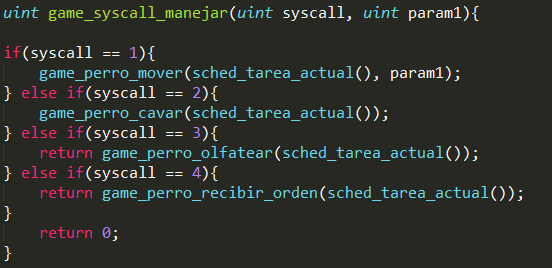
\includegraphics[width=\linewidth]{ejercicio6/syscall_manejar.png}
\caption{{\small \textit{Manejo de interrupciones}}}
\endminipage
\end{center}
\end{figure}

Luego, como el Tp lo pide, es necesario que se salte a la tarea $idle$ por ende cuando se vuelve a la interrupcion 0x46, al final salta a la $idle$ haciendo jmp 0x68:0.

\subsection{item h)}

Este itém lo testiamos y todo anduvo bien, como no va a estar en el tp final borramos el código que lo implementaba, pero fue testiado.



\newpage
\section{Ejercicio 7:}
\subsection{Introducción:}

En este ejercicio realizaremos el \textit{scheduler}.

\begin{itemize}

\item [\textit{a)}]  Construir una función para inicializar las estructuras de datos del \textit{scheduler}.

\item [\textit{b)}] Crear la función  \textit{sched\_proxima\_a\_ejecutar()} que devuelve el  índice de la próxima tarea a ser ejecutada. 

\item [\textit{c)}]  Crear una función \textit{sched\_atender\_tick()} que llame a \textit{game\_atender\_tick()} pasando el número de tarea actual y luego devuelva el índice en la gdt al cual se deberá saltar. Reemplazar el llamado a \textit{game\_atender\_tick} por uno a \textit{sched\_atender\_tick} en el handler de la interrupción de reloj.

\item [\textit{d)}] Modificar la rutina de la interrupción 0x46, para que implemente los servicios según se indica en la sección 4.4.13

\item [\textit{e)}]  Modificar el código necesario para que se realice el intercambio de tareas por cada ciclo de reloj. El intercambio se realizará a según indique la función \textit{sched\_proxima\_a\_ejecutar().}

\item [\textit{f)}]  Modificar las rutinas de excepciones del procesador para que desalojen a la tarea que estaba corriendo y corran la próxima.

\item [\textit{g)}] Implementar el mecanismo de debugging explicado en la sección 4.8 que indicará en pantalla la razón del desalojo de una tarea.

\end{itemize}

\subsection{Ítem a): Inicializar el \textit{scheduler}}

Para incializar el scheduler completamos la funicón \textit{void sched\_inicializar()} del archivo sched.d. En el tp el scheduler es una estructura que posee un array de tareas denimoinado \textit{tasks} y un int denominado \textit{current} en el cual se guarda la tarea actual. Las tareas tambien son estructuras, y contienen un int para recordar la posicion en la que se guarda en la gdt y un puntero a la tarea que representan. Esta estructura se puede obserbar en la siguiente imagen:

\begin{figure}[H]
\begin{center}
\minipage{0.5\textwidth}
 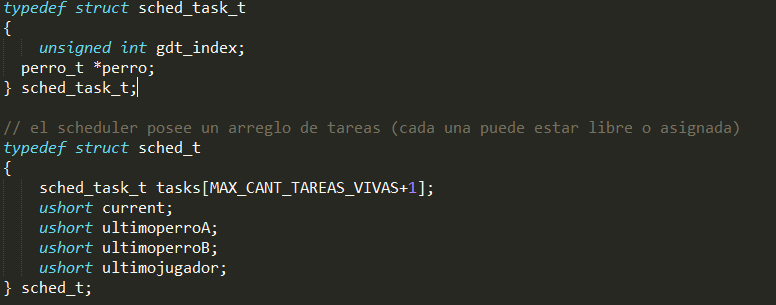
\includegraphics[width=\linewidth]{ejercicio7/sched.png}
 \caption{{\small Estrctura del scheduler usado} }
\endminipage
\end{center}
\end{figure}

La función en cuestión es la siguiente:

\begin{figure}[H]
\begin{center}
\minipage{0.5\textwidth}
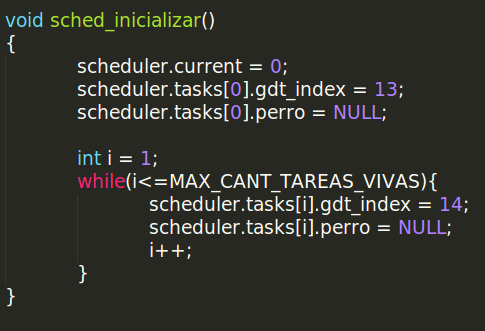
\includegraphics[width=\linewidth]{ejercicio7/funcion.png}
\caption{{\small \textit{void sched\_inicializar()} }}
\endminipage
\end{center}
\end{figure}

Para inicializar la estructura del scheduler realiza lo siguiente:

\begin{itemize}

\item [\textit{A}] Setea el valor de \textit{current} en 0, pues la tarea inicial debe ser la tarea \textit{IDLE} y por convención decidimos que esta se encuentre en la posición 0 del array de tareas. Devido a la decisión anterior, setiamos en el vector de tareas que el gdt\_index de la tarea 0 sea 13 (posición en la \textit{GDT} de la tarea \textit{IDLE} ) y que el puntero a la tarea de la tarea 0 sea \textit{NULL}.

\item [\textit{B}] Luego itera por todo el array de tareas \textit{tasks} seteandole a cada tarea una posición en la gdt correspondiente y seteando el puntero decada una en \textit{NULL}.

\end{itemize}

\subsection{Ítem b):  Crear la función  \textit{sched\_proxima\_a\_ejecutar()}}

Esta función comienza guardando cual es el jugador de la tarea actual y busca las siguiente tarea que corresponda al suiguiente jugador. Para esto itera por todas las tareas y se fija entre las que no tienen un puntero a una tarea \textit{NULL} si alguna pertence al jugador contrario, en caso de que no la encuentre busca devuelta entre todas las tareas pero solo fijandose si no tienen un puntero a una tarea  \textit{NULL}.

\begin{figure}[H]
\begin{center}
\minipage{1.00\textwidth}
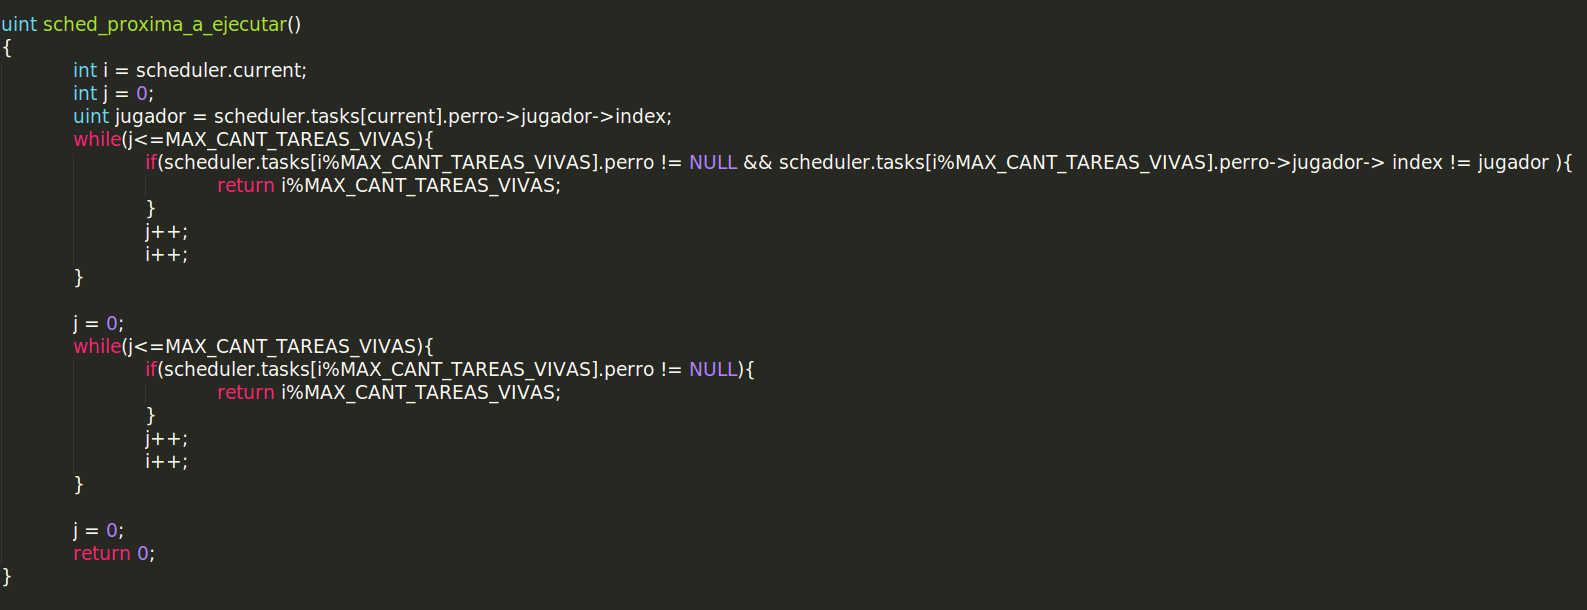
\includegraphics[width=\linewidth]{ejercicio7/proxeje.png}
\caption{{\small \textit{Funcion proxima tarea a ejecutar }}}
\endminipage
\end{center}
\end{figure}

\subsection{Ítem c):  Crear una función \textit{sched\_atender\_tick()}}

Esta función debería devolver la posicion de la \textit{GDT} de la proxima tarea, para eso utiliza la funcion del item anterior, además actualiza el int \textit{current} de la estructura del sheduler. 

\begin{figure}[H]
\begin{center}
\minipage{0.8\textwidth}
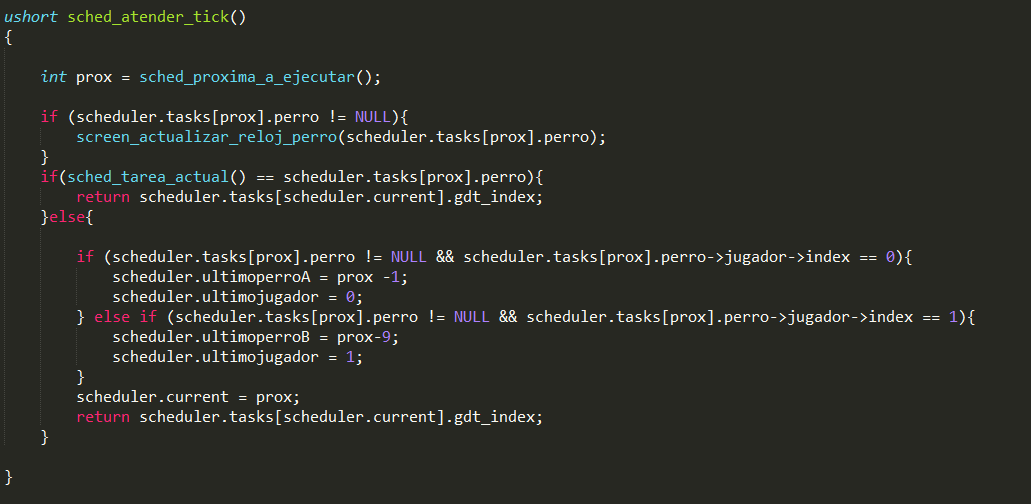
\includegraphics[width=\linewidth]{ejercicio7/atendtick.png}
\caption{{\small \textit{Funcion proxima tarea a ejecutar }}}
\endminipage
\end{center}
\end{figure}

\subsection{Ítem d):  Atender la interrupcion 0x46}

\subsection{Ítem e):  Realiza el intercabio e tareas}

El intercambio de tareas lo realizamos en cada interrupción del reloj, utilizando las funciones explicadas anteriormente. Para utilizarlas escribimos las siguientes lineas en la \textit{RAE} del reloj:

\begin{center}

    pushad \\    
    call fin\_intr\_pic1 \\
    call sched\_tarea\_actual \\
    push eax    \\
    call game\_atender\_tick \\           
    call sched\_atender\_tick \\

    str cx \\
    cmp ax,cx \\
    je .fin \\
    mov [selector], ax \\
    jmp selector:offset \\

    .fin: \\
     call screen\_actualizar\_reloj\_global \\    
    pop eax \\
    popad \\
    iret \\

\end{center}

Esta rutina pregunta por la poscicion de la \textit{GDT}  de la proxima tarea a ejecutar y si la proxima tarea a ejecutar es la misma que se esta ejecutando ahora no hace nada, sin embargo si es diferente realiza un \textit{jmp far} utilizando como selector la posicion en la \textit{GDT} correspondiente. De esta forma se  guarda la \textit{TSS} actual y se carga la nueva. 








\end{document}


